\begin{table*}[t]
  \begin{subtable}[t]{\columnwidth}
    \begin{tabularx}{\columnwidth}{Xr@{\hspace{0.5in}}Xr}
    \multicolumn{4}{c}{\textbf{Gender}} \\
    \midrule
    Female & 51 & Male & 140 \\[0.1in]
    \multicolumn{4}{c}{\textbf{Age}} \\
    \midrule
    Under 18 & 12 & 30--34 & 15 \\
    18--19 & 74 & 35--39 & 6 \\
    20--21 & 12 & 40--49 & 13 \\
    22--24 & 22 & 50--59 & 7 \\
    25--29 & 29 & 60+ & 1 \\
    \end{tabularx}
    \caption{\textbf{2012--2013}, 191 participants.}
  \end{subtable}
  \begin{subtable}[t]{\columnwidth}
    \begin{tabularx}{\columnwidth}{Xr@{\hspace{0.5in}}Xr}
    \multicolumn{4}{c}{\textbf{Gender}} \\
    \midrule
    Female & 127 & Male & 122 \\[0.1in]
    \multicolumn{4}{c}{\textbf{Age}} \\
    \midrule
    Under 18 & 0 & 31--35 & 35 \\
    18--20 & 12 & 36--40 & 28 \\
    21--24 & 21 & 41--50 & 52 \\
    25--26 & 19 & 51--60 & 34 \\
    27--30 & 34 & 60+ & 9 \\
    \end{tabularx}
    \caption{\textbf{2013--2014}, 288 participants.}
  \end{subtable}
\caption{\textbf{Demographic breakdown of \PhoneLab{} participants.} Date
ranges are inclusive.}
\label{table-demographics}
\end{table*}



\section{The PhoneLab Testbed}
\label{sec-testbed}

\PhoneLab{} began operating in 2012 with 191~participants\footnote{We refer
to people carrying \PhoneLab{} phones and participating in experiments as
\PhoneLab{} \textit{participants}, to differentiate them from researchers
running \PhoneLab{} experiments which we call \textit{users}.} using
Nexus~S~4G smartphones~\cite{nexuss4g} running Android
4.1.1~\cite{jellybean}. The first year of operating was a beta test allowing
us to develop the software and expertise necessary to manage a large testbed.
No external experiments were solicited, but several internal experiments were
performed including a usage characterization study that produced the results
described in Section~\ref{sec-experiments}. In 2013, \PhoneLab{} grew to
288~participants using Samsung Galaxy~Nexus devices~\cite{nexuss4g} running
Android 4.2.2. Participants receive discounted voice, data, and messaging
from Sprint in exchange for their participation, and are required to use
their \PhoneLab{} phone as their primary device.

\PhoneLab{} experiments are either distributed through the Play Store or as
platform over-the-air (OTA) updates. Participants are notified of new
experiments and choose whether to participate after reviewing what
information will be collected about them. \PhoneLab{} participants are
\textit{required} to participate in experimentation but \textit{not required}
to participate in any particular experiment. They may remove experiments that
they deem too intrusive or that negatively affect their device. Some
experiments may run in the foreground and interact with users like typical
applications, while others may gather data silently in the background.

\PhoneLab{} users must provide human subjects review documentation, a list of
log tags to capture (which we describe later in this section), and their
experimental software---either a link to the Play Store or a patch against
the current \PhoneLab{} platform source.  Experiments generate data through
the standard Android logging interface. Log messages generated by \PhoneLab{}
experiments are captured and uploaded to a central server while the device is
plugged in and charging. When experimentation completes, the user receives an
archive containing every log message matching their tags generated by all
participating devices.

\begin{table}[t]

\begin{tabularx}{\columnwidth}{Xrr}
\multicolumn{1}{c}{\normalsize{\textbf{Tag Name}}} & 
\multicolumn{1}{c}{\normalsize{\textbf{Tag Count}}} & 
\multicolumn{1}{c}{\normalsize{\textbf{\%}}} \\
\toprule
\texttt{ActivityManager} & \num{96251731} & 13.7 \\
\texttt{dalvikvm} & \num{92565828} & 13.1 \\
\texttt{ConnectivityService} & \num{19195475} & 2.7 \\
\texttt{ActivityThread} & \num{17447815} & 2.5 \\
\texttt{PhoneStatusBar} & \num{13823998} & 2.0 \\
\texttt{SizeAdaptiveLayout} & \num{9857534} & 1.4 \\
\texttt{wpa\_supplicant} & \num{9279597} & 1.3 \\
\texttt{System.err} & \num{8141399} & 1.2 \\
\texttt{SAN\_SERVICE} & \num{7530577} & 1.1 \\
\texttt{LocationManagerService} & \num{6640001} & 0.9 \\
\texttt{DexLibLoader} & \num{5438086} & 0.8 \\
\texttt{SecCamera} & \num{5436968} & 0.8 \\
\texttt{HeartbeatService} & \num{4871085} & 0.7 \\
\texttt{Beautiful Widgets(4120000)} & \num{4692578} & 0.7 \\
\texttt{AudioCache} & \num{4447544} & 0.6 \\
\texttt{k9} & \num{4330848} & 0.6 \\
\texttt{SensorActivatorService} & \num{4177370} & 0.6 \\
\texttt{ThrottleService} & \num{4121301} & 0.6 \\
\texttt{VoldCmdListener} & \num{4014302} & 0.6 \\
\texttt{WindowManager} & \num{3948168} & 0.6 \\
\texttt{AudioHardware} & \num{3913724} & 0.6 \\
\end{tabularx}

\caption{\textbf{Top 20 log tags generated by Android.} During 21~days
\PhoneLab{} collected \num{704216410} log messages from \num{7556} tags.}

\label{table-logtags}

\vspace*{-0.1in}
\end{table}


\subsection{Platform and Device}

\PhoneLab{} phones run the popular Google Android Open-source Smartphone
Platform (AOSP). Using an open-source platform for \PhoneLab{} was an obvious
choice for obvious and less-obvious reasons. The obvious reason is that the
AOSP allows \PhoneLab{} users to experiment with any software component,
meeting our goal of providing a powerful testbed. Modifications to Android
services that provide location, access networks, and manage power can be
benchmarked alongside unmodified devices. Of course, power also creates
problems: faulty experiments can render phones inoperable and threaten
participation. As a result, experimentation at the platform level will
require additional pre-deployment testing and interaction with the
\PhoneLab{} team when compared with experiments that only distribute novel
applications or collect data at the application level. We plan to begin
supporting external platform experimentation in 2014.

We have also found that using an open-source platform has other, less obvious
benefits. First, the availability of the Android source makes \PhoneLab{}
instrumentation easier even when collecting data from the application level
because it gives a visibility into hidden APIs. For example, our usage
characterization experiment, described in Section~\ref{sec-experiments}, uses
Java reflection to access hidden battery usage APIs. Second, using the AOSP
allows us to sign the platform image used by our participants. When the same
key is used to sign a software package, that application may run as the
system user with root privileges. Using this feature allows us to distribute
and update core \PhoneLab{} experimental management software via the Play
Store while retaining the privileges necessary to collect logs and perform
platform updates.

Finally, we expect that our base \PhoneLab{} platform image will evolve to
meet the needs of the research community. While we have found that Android
already logs a wealth of information about platform operation, there are
places where more information could be exposed or logged in a more
experiment-friendly way. Controlling the platform provides the opportunity to
supplement existing interfaces or add additional logging to facilitate
experimentation.

We distributed Samsung Nexus~S~4G smartphones to our first year of
participants and Samsung Galaxy~Nexus smartphones to our second year. Both
were official AOSP development phones and are well-supported, although we had
to obtain proprietary drivers directly from Sprint for the Galaxy~Nexus.
While we expect to receive yearly phone upgrades and will distribute a more
up-to-date device to our second group of participants, we anticipate that the
prohibitive cost of the newest flagship smartphones will prevent us from ever
deploying them on \PhoneLab{}.

\begin{table*}[t]

\begin{tabularx}{\textwidth}{rrrX}
\multicolumn{1}{c}{\normalsize{\textbf{Tag Name}}} & 
\multicolumn{1}{c}{\normalsize{\textbf{Tag Count}}} & 
\multicolumn{1}{c}{\normalsize{\textbf{\%}}} & 
\multicolumn{1}{c}{\normalsize{\textbf{Description}}} \\
\toprule
\texttt{PhoneLabSystemAnalysis-Snapshot} & \num{4507143} & 71.8 & Collects battery breakdown across components and applications. Polled every 15 minutes. \\
\texttt{ActivityManager} & \num{1078872} & 17.2 & Logs application management actions. \\
\texttt{PhoneLabSystemAnalysis-Telephony} & \num{240882} & 3.8 & Records phone call state and radio signal strength. \\
\texttt{PhoneLabSystemAnalysis-BatteryChange} & \num{212929} & 3.4 & Logs every change to the battery level. \\
\texttt{PhoneLabSystemAnalysis-Wifi} & \num{144163} & 2.3 & Logs connection state, scan information and signal strength. \\
\texttt{LocationManagerService} & \num{45478} & 0.7 & Records when GPS is enabled and disabled. \\
\texttt{PhoneLabSystemAnalysis-Location} & \num{26588} & 0.4 & Passively logs all location updates. \\
\texttt{PhoneLabSystemAnalysis-Misc} & \num{20960} & 0.3 & Logs when the screen turns on and off. \\
\texttt{SmsReceiverService} & \num{2686} & 0.0 & Used to count text messages sent and received. \\
\texttt{PhoneLabSystemAnalysis-Packages} & \num{112} & 0.0 & Records when
applications are installed and removed. \\
\end{tabularx}

\caption{\textbf{Log tag statistics for one day during our
experiment.} \num{6279813} total log tags were collected.}

\label{table-experimenttags}

\end{table*}


\subsection{Participants}

Recruiting a large number of \PhoneLab{} participants requires effective
incentives. In their first year of \PhoneLab{} participation, voice, data and
messaging are free with funding provided by the National Science Foundation
(NSF). This free year of service plays a major role in our recruiting
efforts. In subsequent years, participants pay a deeply discounted \$45 per
month rate for unlimited data and messaging through a deal negotiated with
Sprint. Sprint has proved to be an ideal partner for the \PhoneLab{} project,
both helpful with testbed logistics and still providing unlimited data plans,
negating any economic impact of our data collection.

Because participants may leave at any time, the front-loaded cost structure
of our incentives makes it most efficient to recruit participants who will be
able to continue as part of \PhoneLab{} for multiple years. While we
anticipate that some participants will leave after the first free year,
interviews with them will help us identify long-term participants during
subsequent years. Long-term participants allow us to amortize the first free
year and provide a stable group comfortable being a part of \PhoneLab{}
experimentation.

When recruiting our first batch of 2012--2013 participants, we targeted
freshman, sophomores, and new PhD students. The University at Buffalo has a
large international graduate student community, and many of these students
arrive on campus without phones or phone contracts, making them ideal
\PhoneLab{} participants. Unfortunately, retention after our first year was
poor: only 43~of~191 first-year participants chose to continue after the free
year ended. We believe multiple factors are at play. First, we now consider
our decision to recruit undergraduates to be a mistake, since many of these
students still have the option of continuing on family plans paid for by
their parents. Second, multiple participants have complained about poor
Sprint coverage, which, while out of our control, is a concern in our area.

As a response to our low first-year retention, during the second year we
targeted staff and faculty along with incoming PhD students and did not
recruit or accept undergraduates. We hope that adult staff members are more
accustomed to paying for phone service and less likely to have a free family
plan to return to. This change to our recruitment focus has also had the
benefit of significantly improving both the gender and age diversity of our
participant pool. As shown in Table~\ref{table-demographics}, while our
first-year participants were primarily young men, our second-year
participants are a good mix of ages and genders, making results more
representative.

\subsection{Testbed Software}

\PhoneLab{} smartphones are distributed with a small piece of testbed
management software integrated into the Android platform. This heartbeat
service uploads periodic reports including information about device location,
battery levels, and the installation status of other required \PhoneLab{}
software. This information is only used for testbed management and never
released to researchers.

On boot, the heartbeat service starts the \PhoneLab{} Conductor, the primary
\PhoneLab{} configuration and data collection tool. Experimental
configuration, log collection, data upload and platform updates are performed
by the Conductor, which is installed and updated through the Google Play
Store. By signing it to match the platform build key it runs with root
privileges, necessary to collect logs from all applications, perform platform
updates, and start experiments that lack a foreground activity. Periodically,
the Conductor retrieves an XML configuration the \PhoneLab{} server. The
configuration specifies what background experiments to start or stop, which
log tags to collect, and the upload policy and endpoints. The Conductor also
uploads status information to the server during the configuration exchange,
including version numbers of \PhoneLab{} software, what experiments are
currently running and how much data is queued for upload.

\PhoneLab{} logging and data collection must be unintrusive. If it is not,
either our participants will quit, or their usage patterns will be affected.
We believe that we have achieved this goal. Measured battery usage of
\PhoneLab{} software is low. A conservative estimate that includes all of the
applications that run as the shared system user comes to a per-participant
average of 2.4\%. Given that this estimate includes many non-\PhoneLab{}
applications that also run as the system user, it should be considered a
strict maximum. Our default policy of only uploading while the device is
charging reduces the overhead of the most power-hungry task. In addition, we
have received no complaints about our tools, even from participants that
initially used their phones without them.

\begin{figure*}[t]

\centering
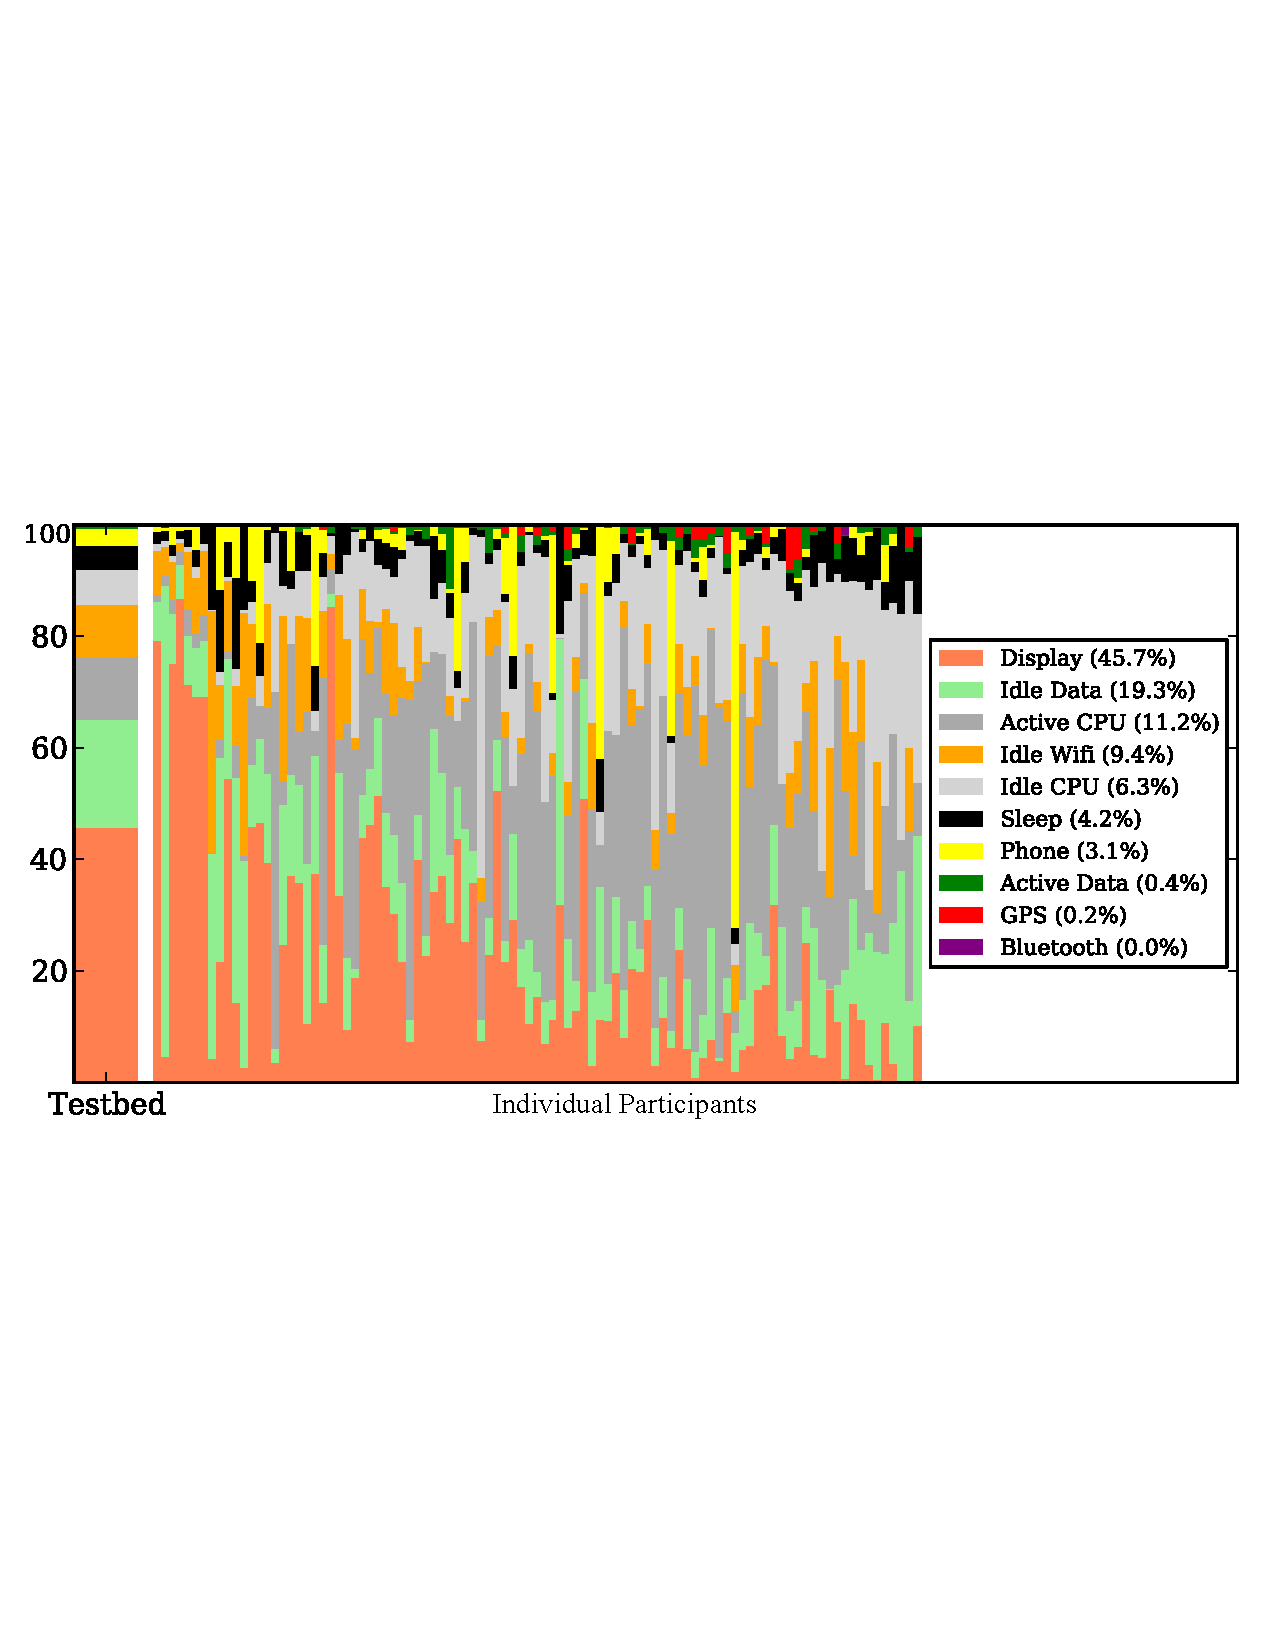
\includegraphics[width=0.8\textwidth]{./figures/power/breakdown/graph.pdf}

\caption{\textbf{Power usage by component.} The large bar at left shows an
aggregated breakdown for all participants. The participant bars are scaled
against the participant with the most energy usage.}

\label{figure-batteryoverview}
\end{figure*}

\subsection{Safety and Privacy}

There is an important difference between \PhoneLab{} and other testbeds, such
as Emulab~\cite{white:osdi:2002}, PlanetLab~\cite{peterson:ccr:2003},
MoteLab~\cite{werner-allen:ipsn:2005}, or
OpenCirrus~\cite{avetisyan:computer:2010}: our experiments involve real
people. There are two core requirements regarding our participants. First,
they should use their phone as they normally would, which motivated the
design of unintrusive testbed management software. Second, and more
importantly, they must feel safe while participating in \PhoneLab{}
experiments.

To accomplish this, we leverage several existing safety mechanisms when
possible. First, we require an Institutional Review Board (IRB) to review
each \PhoneLab{} experiment for human subjects compliance. IRB approval or an
official exemption is required before any \PhoneLab{} any experiment can begin.

Second, we distribute experimental applications to a group of developers
prior to broader release, allowing us to identify any significant problems
before they reach our participants. This step is particularly important for
platform experiments, which must be established as stable before being
distributed.

Finally, we utilize Android's existing safety and privacy mechanisms.
Participants are presented with the typical Android privacy dialog during
experiment installation. Rather than building an alternate distribution
channel or privacy mechanism, we felt it was sufficient and probably better
to use a process participants are familiar with. After installation, if a
participant discovers that an experiment malfunctions or wastes power, they
can uninstall it. If we notice patterns of experimental removal, we will flag
the experiment and notify the researcher.

\subsection{Experimental Procedures}

To conclude, we review \PhoneLab{} experimentation from a researcher's
perspective. First, develop your application locally. Any information logged
through the standard Android logging library can be recorded. In addition,
the platform may already be logging useful information for you. Keep track of
all the log tags you want \PhoneLab{} to capture. Approach your local IRB and
receive experimental approval and upload your application to the Play Store.

Second, upload your list of log tags, IRB letter, and link to your
application on the Play Store through the \PhoneLab{} website. We will
contact you when we begin beta testing and again once your experiment is
ready for the testbed. During beta testing you will be provided with
\PhoneLab{} log output to ensure that your experiment is running properly.

Finally, your experiment will be scheduled. Our goal is to maintain a
medium-sized list of active experiments for our participants: large enough to
make good use of the testbed, but small enough to ensure that each experiment
is picked up by many participants. When your experiment completes, you will
receive a archive with messages matching the tags you selected.
